\subsection{XmlMarshaller}
XmlMarshalleren er en klasse der implementerer IProtocolMarshal interfacet, Der vil i fremtiden være flere af disse protokol marshallers så den sendte kode kunne være andet end XML, men da det var fokuspunktet for dette projekt er der kun skabt denne ene. Dog med et interface så der stadig er mulighed for at udbygge systemet. XmlMarshalleren har til ansvar at fjerne postfix navnet "Cmd" fra det objekt der er kaldt enten encode eller decode på, Og vil så herefter søge i \gls{SL}'s mappestruktur efter en lignende klasse blot med postfix "Marshal", hvis denne findes vil der blive kaldt den givne kommando, (enten encode eller decode) på denne marshaller. Hvis ikke marshalleren findes vil der tilgengæld blive smidt en exception med en meddelelse om at marshalleren ikke findes. 

\begin{figure}[H]
	\centering
	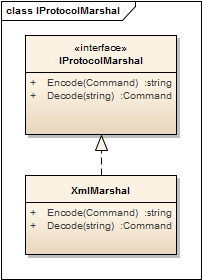
\includegraphics[width=0.4\textwidth]{Systemdesign/SharedLib/Images/Klasser/IProtocolMarshal.png}
	\caption{XmlMarshal der implementerer IProtocolMarshal}
	\label{fig:klasseXmlMar}
\end{figure}
